\documentclass{report}
\usepackage{amsmath}
\usepackage{caption}
\usepackage{subcaption}
\usepackage{verbatim}
\usepackage{amssymb}
\usepackage{graphicx}
\usepackage{url}
\usepackage{booktabs}
\usepackage{cleveref}

\DeclareMathOperator*{\argmax}{argmax}
\DeclareMathOperator*{\argmin}{argmin}

\title{\Huge \textbf{RSMG Progress Report 1}}
\author{David McDonald \\
	Superviser: Dr. Shan He}
\date{}

\begin{document}
	
	\maketitle
	
	\tableofcontents
	
%	\begin{abstract}
%		Do I need an abstract?
%	\end{abstract}
	
	\chapter{Introduction}
	
	The overall goal of my PhD is to construct a complex network model of biological data, by combining gene expression levels, known pathways, protein interactions and known semantic information. Then, through feature learning techniques, use inference to generate testable hypotheses from this model about the complex and still largely unknown interactions that comprise the world in which we live. This can be broadly broken down into two areas: complex network analysis and feature learning. 
	
	A complex network is a graph that is comprised of non-trivial or uniform features. These networks often arise when modelling real-word systems. The early belief was that the interactions of such seemingly unrelated things as proteins, social interactions and the internet were random and unconnected. However, it has been shown that most real world systems have the same basic architecture \cite{barabasi2009scale}. Real world networks often scale-free in that the distribution of node degree is a power law. Connections are preferentially made between nodes with a probability proportional to their existing degree. Some complex networks also are characterised by the `small world' phenomenon, where one would expect a small average shortest path length and a high degree of clustering \cite{watts1998collective}. The underlying similarity of the interactions between agents in real-world phenomena is surprising and launched the popularity of complex network research. Research that has swiftly captured the imagination of researchers of many fields; fields such as epidemiology, mathematics, computer science, sociology and biology.
	
	Feature learning comprises a set of machine learning techniques that extract useful features from raw data. These features aim to model the underlying constructs of the data and can be used as the first step of more complex machine learning tasks, such as classification. The recent boom in popularity of deep learning and advent of efficient training algorithms has lead to deep models designed te hierarchically extract features from the data. For example, in the landmark computer vision paper of 2012, Krizhevsky et al. \cite{krizhevsky2012imagenet} trained a deep convolutional neural network to extract hierarchically features from colour images, achieving state-of-the art results. Visualisation of the trained filters shows that the network was, indeed, extracting features hierarchically, the first layer looked for edges, the next for shapes etc. This is analogous to how the human brain processes images.
	
	Generative models, such as the Restricted Boltzmann Machine (RBM), suppose that there are hidden latent variables controlling the data and aim to use inference to learn the distribution of the data. RBMs suppose a conditional independence between components of a particular observance of the data, and between the hidden, latent variables. This allows for very efficient training algorithms such as the Geoffrey Hinton's contrastive divergence algorithm \cite{hinton2002training}. However, by adding intra-level connections between the hidden latent variables, we can also learn the relationships between these variables. 
	
	While feature learning commonly involves reducing the dimension of the data by condensing a large dataset to a small number of features, actually allowing for a number of features much larger than the dimension of the original data. By imposing a sparsity constraint on the latent representation of the data, such that the expected output of a particular hidden unit is close to 0, sparse coding is able to learn a `dictionary' of codes whereby a particular data point is composed of few of these codes.
	
 

	\chapter{Community Detection in Complex Networks}

	Most real-world complex networks contain subsets of nodes that contain a higher degree of inter-connectivity than the rest of the network
	% \cite{palla2005uncovering}. 
	\cite{lancichinetti2009detecting}.
	These subsets are commonly referred to as communities. 
	A rigorous definition for a `community' within a network still seems to elude the scientific community \cite{lancichinetti2009detecting}.
	However, the most popular definition among scholars is the planted l-partition model. 
	This was popularised thanks to Girvan and Newman in their seminal work \cite{girvan2002community} and states that as long the probability of a node being connected to its group is greater than the probability of it being connected to the rest of the graph, then those groups are communities. 
	
	`Community detection' is the name given to the problem of finding the underlying community structure in a given network \cite{girvan2002community}. 
	%Many complex problems can be represented as a network and many large networks modelling real world interactions have been shown to follow the same scale-free power-law distribution \cite{barabasi1999emergence}. 
	Since many complex problems can be represented as a network, community detection has proven to be useful in seemingly disconnected areas of study, such as social \cite{barber2007modularity}, biological \cite{fortunato2007resolution}, and world-wide-web \cite{danon2006effect} analysis.
	
	Most real world networks do not solely contain communities at one scale \cite{lancichinetti2009detecting,yang2013hierarchical}. 
	They contain super communities that may contain sub-communities, that may, in turn, contain their own sub communities.
	And so on. 
	Delving deeper into the community structure may offer some insight into how these processes work.
	%For example, a network of interest in a scientific paper may contain super communities corresponding to the scientific community, hobbyists and the author's own friends and family. 
	%Zooming in on the scientific community, one may notice sub-communities of various related academic disciplines such as Mathematics, Biology, and Physics. 
	%Uncovering the multiple levels of community structure in the network can provide more information from the same underlying data than finding only communities at one level. 
	For example, hierarchical analysis of protein-protein interaction networks may help to identify subsets of functionally-related proteins that interact together strongly within an established community representing some biological process.
	
	%TODO gap in field
	But, a general community detection algorithm does not yet exist.
	Many existing algorithms suffer from a number of issues. 
	To name a few:
	The number and scale of communities must be known a-priori, which in most real applications, is infeasible.
	Additionally, the relationships between communities, both one the same level and at different ones, is lost.
	Identifying not only the community itself, but its position in the network as a whole, provides further insight into the often abstract interactions that comprise complex networks and so preserving this information when analysing a network is paramount.
	And, in some cases, the algorithms cannot deal with special cases: for example, modularity-based methods suffer from the so-called `resolution limit' \cite{fortunato2007resolution}.
	
	The Growing Hierarchical Self-Organizing Map (GHSOM), which was first described by Dittenbach et al. \cite{dittenbach2000growing},
	% and then expanded upon in  \cite{dittenbach2002uncovering,rauber2002growing}, 
	offers a unique solution to these problems .
	It uses the topology-preserving property of self-organizing maps, in conjunction with the ability for maps to grow into arbitrary shape completely autonomously. 
	GHSOM is capable of detecting the community structure of complex networks and adapt the shape of its maps to fit the structure of the data.  
	And, by selecting promising areas of the input space to expand and produce maps of finer granularity, GHSOM is capable of studying interesting areas of  the input space in greater detail.
	%These properties suggest that GHSOM might be a suitable choice for a general tool for detecting communities in biological networks that so commonly feature a hierarchical structure. 
	%Preserving the topology of the input space will produce a map of communities that shows the how the communities link together and super and sub community relationships in the network.
	These properties suggest that GHSOM is a suitable candidate for a hierarchical community detection algorithm, and this study will explore the usefulness of GHSOM for this task.

	\section{Related Work}
	Over the years, numerous and varied approaches have arisen to tackle the problem of community detection. 
	Readers interested in thorough reviews and in-depth algorithm comparisions are directed to  \cite{fortunato2010community}.
	
	\subsection{Cut-Based and Spectral Approaches}
	Most early work on community detection focused on `cutting' the network into modules, in such a way that the number of edges cut was minimized. 
	In theory, this resulted in the best partition of the network into communities \cite{kernighan1970efficient}.
	%However, this often favoured cuts of small, peripheral subgraphs, so it was adapted into ratio cut \cite{wei1991ratio}, normalised cut \cite{shi2000normalized} and min-max cut \cite{ding2001min} that took the number of nodes in each resulting sub-graph into account, and thus resulted in a partition that was more balanced.
	However, this often favoured cuts of small, peripheral subgraphs, so it was adapted into ratio cut, normalized cut and min-max cut that took the number of nodes in each resulting sub-graph into account, and thus resulted in a partition that was more balanced.
	Summaries of these cuts can be found in \cite{fortunato2010community}.
	%\begin{align}
	%Rcut(A_1,...,A_k) = \sum_{i=1}^K \frac{cut(A_i,\bar{A_i})}{|A_i|}
	%\end{align}
	
	%More recently, `conductance' has become a common term for defining a good cut. 
	%Conductance, defined as:
	%\begin{align}
	%\phi(S) = \frac{c_s}{\min(Vol(S),Vol(V \setminus S)} 
	%\end{align}
	%with
	%\begin{align}
	%c_s = |\{(u,v) : u \in S, v \not\in S\}|
	%\end{align}
	%is concerned with edges, rather than vertices, and has been used to detect communities in bipartite networks \cite{barber2007modularity} and combined with PageRank \cite{andersen2006local}. 
	
	Spectral clustering dates back to the work of Donath and Hoffman in 1973 \cite{donath1973lower}. 
	However, it was popularized in the early 2000s \cite{ng2002spectral}. 
	%However, it was popularized by the works of Shi and Malik \cite{shi2000normalized}, Ng et al. \cite{}, and Ding \cite{ding2004tutorial}.
	Spectral methods rely upon constructing `Laplacian' matrices from the raw network data and eigen-decomposing them. 
	Clustering the resulting eigenvectors results in clusters of the original data points. 
	Spectral approaches have many advantages over other techniques and, as a result, they have become popular in the machine learning community for clustering  on non-linear manifolds. 
	%According to \cite{von2007tutorial}, `these methods do not make assumptions about the form of the clusters' and are capable of correctly identifying typically challenging clusters, such as the famous two spirals example. 
	%For community detection, they have the additional benefit of efficiency, especially if the graph adjacency matrix is sparse. 
	%They are also able to detect which nodes form connected components within a general network where nodes are not always connected \cite{von2007tutorial}. 
	Spectral methods can also be combined with traditional hierarchical modularity methods \cite{donetti2004detecting}.
	% where the graph was eigen-decomposed and projected into a $g$-dimensional subspace and then the resulting points were clustered to maximize modularity.
	
	%\subsection{Evolutionary Approaches}
	%Approaches using evolutionary algorithms typically encode the community structure of a graph using the locus based adjacency first proposed in \cite{park1998genetic}. The genotype consists of $N$ genes and $j$ appearing in gene position $i$ is interpreted as nodes $i$ and $j$ belonging to the same community. This representation was used to great effect as part of the MOCK algorithm \cite{handl2007evolutionary} which solved the community (or in this case, clustering) problem using a multi-objective optimisation algorithm that attempted to balance compactness and connection of the clusters, and used several novel genetic operators. Variation modifiers are used in \cite{pizzuti2008ga} to reduce the search pace by taking into account the correlations of the nodes.
	
	
	
	%Further early work includes the Metis algorithm \cite{karypis1998fast}, that finds the best split of a graph into two equal sized pieces, and the MQI algorithm \cite{gallo1989fast}. 
	Further work includes the Markov Clustering algorithm (MCL) that simulates a diffusion process on a graph by repeatedly performing stages of expansion and inflation and only keeping the $k$ largest elements for efficiency \cite{van2001graph}. 
	%His algorithm has since found use in Miru, a commercial 3D network visualization software, to cluster very large graphs quickly.
	
	\subsection{Modularity-Based Approaches}
	The seminal work of Girvan and Newman \cite{girvan2002community} marked a significant advance in the field by providing the first quantitative measure of a community: modularity. 
	The modularity of a partition of a network 
	%defined as
	%\begin{align} 
	%\label{modularity}
	%Q = \sum_{s=1}^m \bigg[ \frac{l_s}{L} - \bigg( \frac{d_s}{2L} \bigg)^2\bigg]
	%\end{align}
	scores a network partition by comparing the number of links inside a given module with the expected number that would be found in a random graph of the same size and degree sequence. 
	%Here, $m$ is the number of modules in the partition, $l_s$ is the number of links in module $s$, $L$ is the total number of links in the network and $d_s$ is the total degree of the nodes in $s$. 
	%The first term in equation \ref{modularity} is the fraction of links inside $s$ and the second term represents the expected fraction of random links in the graphs to be in the module. 
	Girvan and Newman propose a hierarchical divisive algorithm that removes edges based on their `betweenness' (the number of shortest paths from two nodes in the network that go through them) until the modularity quality function is maximized. 
	The early work of Girvan and Newman has since been expanded upon.
	For example, edge clustering in favour of edge-betweenness \cite{radicchi2004defining}, iteratively adding links to a module based on their expected increase in modularity \cite{clauset2004finding}, and multi-stage local optimization \cite{blondel2008fast}.
	
	%Radicchi at al. \cite{radicchi2004defining} used a similar divisive algorithm, but instead of edge betweenness, used an edge clustering co-efficient based on loops in the network. 
	%They also proffers the notion of `strong' and `weak' communities based on their internal and external degrees. 
	%Clauset et al. \cite{clauset2004finding} sped up Newman's the agglomerate algorithm in \cite{newman2005power} to iteratively add links to a module based on their expected increase in modularity. 
	%A similar approach was performed by Guimera and Amaral \cite{guimera2005functional} with simulated annealing. 
	%Blondel et al. \cite{blondel2008fast} offered a multi-stage local optimization of Girvan and Newman's algorithm that iteratively replaced communities with a single node. 
	
	%Other work with modularity-based quality scores include the work of Rosvall and Bergstrom \cite{rosvall2007information} that translated the problem of community detection into the problem of optimally compressing the information in a graph such that the most information can be uncovered when the compression is decoded. 
	%They used simulated annealing to minimize a function that represented both compression and data loss. 
	%While slow and computationally expensive, this approach was also shown to work well with dynamic processes in his later work \cite{rosvall2008maps}. 
	
	%It has been shown that modularity-based approaches have their limitations. 
	%In particular, Fortunato and Bartelemy \cite{fortunato2007resolution} show what they referred to as the `resolution limit' - that modularity-based approaches can fail to identify communities that are smaller in size than a scale that depends on the size of the network, and this results in incorrect community division in the cases when even small communities must be considered. 
	%But it has been shown that resolution limit can be overcome.
	%Ronhovde and Nussinov \cite{ronhovde2010local} does not compare to a null model as in equation \ref{modularity}, but instead penalize communities for any missing edges. 
	%This provided good results even on very small communities compared to the size of the overall network. 
	
	\subsection{Statistical Approaches}
	Statistical approaches have been shown to deduce the best model to fit the data represented in the graph structure, which may not necessarily be communities \cite{newman2004finding}.
	They have also been used to show the trade off between using heuristics to reduce the search space and optimization of a constrained quadratic function \cite{yang2013hierarchical}.
	%In \cite{newman2004finding}, Newman and Girvan used Bayesian inference to deduce the best model to fit the data represented in the graph structure.
	%His algorithm was capable of finding the best group structure for any graph, no just a community structure, but required the number of groups to be know a-priori. 
	%Probability theory was also used by Yang et al. in \cite{yang2013hierarchical} for the construction of their Probabilistically Mining Communities (PMC) algorithm. 
	%PMC offers a trade off between using a random walk as a heuristic to reduce the search space and optimizing using a constrained quadratic optimization function. 
	%Furthermore, `label propagation' methods proposed by Raghavan in \cite{raghavan2007near} have had success at detecting communities in real time \cite{leung2009towards}.
	
	
	\subsection{Neural Network Approaches}
	The deep learning community has began to explore the possibilities of using neural networks for clustering in the graph domain. Convolutional neural networks (CNNs), powerful machine learning tools that have proven very successful for challenging classification tasks that have recently been generalised to take a graph input \cite{defferrard2016convolutional}. 
	CNNs have also been used for semi-supervised learning on graphs, where the they are capable of learning both graph structure and node features \cite{kipf2016semi}. 
	%Here, some nodes are labelled the labels of every other node are inferred by the model, which is capable of learning both the graph structure and node features.  
	
	\section{Hierarchical Community Detection}
	%In many practical networks, partitioning a network into a cover does not accurately reflect the inherent community structure of the data. Sometimes, nodes can belong to more than one community -- sometimes communities overlap. The first algorithm to consider overlapping communities was CFinder in 2006 \cite{adamcsek2006cfinder}. Drawing from the earlier work of Palla et al. and the Clique Percolation Method (CPM) \cite{palla2005uncovering}, CFinder considered communities as the unions of k-cliques and so rolled k-cliques across the graph to detect communities. While computationally expensive, it was able to deal with overlapping cases, and opened the door for further study. Shen et al. proposed EAGLE in 2009 \cite{shen2009detect} that used maximal cliques, an agglomerative hierarchical structure and a modified modularity quality function that detected complex overlapping community structures.
	
	The hierarchical nature of modularity-based clustering methods can allow them to detect communities at different scales. 
	\cite{lancichinetti2009detecting} used local optimization to maximize a fitness function with a parameter that controlled the size of communities detected.
	Other work includes multi-scale quality functions that can uncover hierarchical communities and produce several different partitions of a graph, the post-processing of clusters found by hierarchical methods (encoded in a dendogram) \cite{pons2011post}, and Bayesian non-negative matrix factorisation that performs `soft-partitioning' and assigns node participation scores to modules \cite{psorakis2011overlapping}.
	
	
	%Complex networks very often contain communities at different scales -- communities within communities -- and it is informative to investigate the communities identified at different levels of hierarchical algorithms to uncover these. 
	%The first algorithm to look for both overlapping and hierarchical communities was proposed by Lancincetti et al. \cite{lancichinetti2009detecting}, where they aim to locally maximize a fitness function based on the fraction of connections going in and out of a subset of nodes, and a parameter $\alpha$ that controlled the scale of the communities uncovered.
	%\begin{align}
	%f_G = \frac{k_{in}^G}{(k_{in}^G + k_{out}^G)^\alpha}
	%\end{align}
	%where $k_{in}^G$, and $k_{out}^G$ are the total internal and external degree of the nodes going into community $G$, and $\alpha$ controls the size of communities. 
	
	%Potts methods have also shown good tolerance towards communities that overlap. 
	%Both \cite{reichardt2006statistical} and \cite{ronhovde2009multiresolution} look for the ground state of spin and interpret the spin configuration that minimizes energy of spin glass as the underlying community structure of the state. 
	%Due to user-controlled resolution parameters, they are able to identify overlapping and hierarchical communities.
	
	
	\chapter{The Growing Hierarchical Self-Organising Map}
	
	The Growing Hierarchical Self-Organising Map (GHSOM), proposed first in 2000 \cite{dittenbach2000growing} for clustering data points into hierarchical clusters is the main focus of my research for this first six months. In particular, I am investigating its usefulness at community detection in complex networks that often contain an inherent hierarchical structure \cite{lancichinetti2009detecting}. For example, a social network may contain a community corresponding to "academics" that could be further broken up into communities of "computer science", "physics", "biology" etc. Additionally, GHSOM can preserve the topological information of the data it is modelling. Features, such as communities, that are close together in the input space should be close together in the map and so I also aim to investigate cooperation between communities. 
	

	I primarily use two phases: projection and map construction. Projection is concerned with embedding the vertices of the network into $k$-dimensional Euclidean space. GHSOM is then used to construct two-dimensional maps of the community structure of the network at different hierarchies.
	
	\begin{figure}
	\centering
	\includegraphics[height=\textheight]{../overall_algorithm.png}
	\caption{A flowchart providing an overview of the entire algorithm.}
	\label{overall_algorithm}
	\end{figure}
	
	\section{Embedding of Vertices using MDS} 
	Multi-Dimensional Scaling (MDS) was used to first embed the vertices of a given network $\textbf{G}$ onto a Euclidean plane $\textbf{X}\subset\mathbb{R}^k$.
	Explicit MDS was used in favour of running GHSOM on the raw network as MDS embeds based on a similarity  measure than can be changed. The embedding for one measure -- say shortest path distance between nodes in the network-- may result in different communities than for another measure -- semantic similarities of genes, based on enriched GO terms, in a co-expression network. The definition of "community" is not yet rigorous and depends largely on what a researcher is interested in investigating \cite{schaub2016many}, and the ability to extract multiple community partitions based on the same data is desirable.
	
	MDS takes as input a matrix $\textbf{D}$ of distances or dissimilarities and attempts to find an embedding of each point such that the relative distances are preserved. 
	Here, we use the shortest path between two nodes as the metric, as in \cite{yamakawa2006self}. 
	This distance is well defined and finite for all pairs of nodes in the network since $\textbf{G}$ is a connected graph. 
	
	We then use double centring to construct a kernel matrix $\textbf{K}$ from $\textbf{D}$ and eigen-decompose it. 
	In order to prevent the need to specify the dimensionality of the data, $k^*$, a-priori, we determine $k^*$ dynamically as follows:
	\begin{align}
	k^* = \argmax_k \Bigg(\frac{\Sigma_{i=1}^k \lambda_i}{\Sigma_{j=1}^n \lambda_j} \geq 0.95 \Bigg)
	\end{align}
	%holds. 
	This ensures that 95\% of variation is preserved, no matter how many nodes in $\textbf{G}$ there are. 
	Then the $k^*$ largest eigenvalues and their associated eigenvectors are used to compute $\textbf{X}$, giving an $n\times k$ matrix where the $i$th row gives the co-ordinates of node $i$ in $k$-dimensional space.
	
	\section{The Growing Hierarchical Self-Organizing Map}
	Embedding the $n$ nodes into $k$ dimensional space translates the problem of finding communities in a graph to identifying clusters in the Euclidean Space $\textbf{X}$. Since the distance (by whatever metric used) between two nodes within the same community should be smaller than two nodes belonging to two different communities, then all of the nodes within a community should be embedded closely together in $\textbf{X}$.
	For clustering the data points in $\textbf{X}$, we use GHSOM.
	
	\section{Hyper-Parameters}
	GHSOM takes two hyper parameters.
	The first is $\epsilon_{sg}$ and this determines the size of the maps that will be created. 
	The second, $\epsilon_{en}$, determines the granularity of the maps produced, or when the network should grow a new layer. 
	Both of these will be discussed in more detail later in this paper.
	Additionally, GHSOM uses a measure of error, that its creators, Dittenbach et al. \cite{dittenbach2000growing,dittenbach2002uncovering} called Mean Quantization Error (or MQE). 
	Following their example, let the MQE of a single neuron $i$ be denoted $\textbf{mqe}_i$ and the MQE of an entire map $m$ be denoted $\textbf{MQE}_m$.
	
	\section{$\textbf{MQE}_0$}
	GHSOM begins with layer 0 comprising a single neuron map. 
	This neuron is given a weight vector $\textbf{w}$ that points to the centre (the mean) of all the data points:
	\begin{align}
	\textbf{w} = \frac{1}{n} \sum_{i=1}^n \textbf{x}_i
	\end{align}
	The MQE of this neuron (and therefore this first map) is the variance of the data set:
	\begin{align}
	\textbf{MQE}_0 = \textbf{mqe}_0 = \frac{1}{n} \sum_{i=1}^n ||\textbf{w} - \textbf{x}_i||
	\end{align} 
	This is used as a benchmark for all the following layers to beat.
	
	\section{Training the First Layer}
	GHSOM then begins by training the first layer map. 
	The first layer is initialized to just one neuron. 
	The weight of this neuron is initially set to be equal to a random data point. 
	The map is then trained as in the standard SOM algorithm, found in \cite{kohonen1990self} for $\lambda=10000$ epochs.
	
	One training epoch consists of presenting each training pattern (the embedded nodes of $\textbf{G}$) to the map. 
	For each pattern $\textbf{x}$, the `winning' neuron $i^*$ is determined as:
	\begin{align}
	i^* = \argmin_i  ||\textbf{x} - \textbf{w}_i||
	\end{align}
	
	The weights of every neuron in the map are then adjusted to move a little closer to $\textbf{x}$, based on how close to $i^*$ they are in the map.
	\begin{align}
	\textbf{w}_i(t+1) = \textbf{w}_i(t) + \eta(t) h(i, i^*, \sigma(t)) (\textbf{x} - \textbf{w}_i)
	\end{align}
	The weights are adjusted proportionally to the learning rate $\eta(t)$, and the neighbourhood function $h(i, i^*, \sigma(t))$, given by
	\begin{align}
	h(i, i^*, \sigma(t)) = \exp\Bigg(-\frac{||\textbf{r}_i-\textbf{r}_{i^*}||^2}{2\sigma(t)^2}\Bigg)
	\end{align}
	where $\textbf{r}_i$ is the position of neuron $i$ in the map.
	The neighbourhood function preserves the topological ordering of the map, as neurons closer to the winning neuron in the map move towards $\textbf{x}$ more.
	At the end of each training epoch, the order of the training patterns is shuffled. Then the neighbourhood width $\sigma(t)$ is adjusted in the following manner:
	\begin{align}
	\sigma(t) = \sigma_0 \exp \Bigg(-\frac{2 \sigma_0 t}{\lambda}\Bigg)
	\end{align}
	
	Both $\eta(t)$ and $\sigma(t)$ vary with time and decrease as the number of training epochs increases. 
	This allows the movements of the weights to gradually decrease and become fine-tuned.
	
	
	
	\section{Growing the Map}
	The original GHSOM paper describes map expansion by inserting a new row or column of neurons into the map. 
	Since, every neuron represents a community, I elected not to follow this example, as I did not want to over estimate the number of communities in the network. 
	As a result, I grow the map one neuron at a time.
	After $\lambda=10000$ training epochs have passed, every node in $\textbf{G}$ is assigned to the neuron in the map whose weight vector $\textbf{w}$ points closest to it in $\mathbb{R}^k$. 
	Then the $\textbf{mqe}_i$ for each neuron is calculated, as well as the overall $\textbf{MQE}_1$ of the map. 
	If 
	\begin{align}
	\textbf{MQE}_1 \geq \epsilon_{sg} \textbf{mqe}_0
	\end{align}
	then the network is expanded, by inserting a single new neuron into the map, else expansion terminates.
	
	Network expansion largely follows the example of Bernd Fritzke in \cite{fritzke1994growing} and aims to preserve a simplicial structure within the map whenever a new neuron is inserted. 
	This ensures that neurons in the map do not have too many neighbours. 
	Firstly, one must identify the `error unit' $e$ -- the neuron with the greatest error in the map. 
	Then retrieve the list of all of the adjacent neurons (the neighbours) of $e$ in the map.
	A new neuron, $i$ is inserted into the map and assigned a weight vector $v$ equal to a random data point that is assigned to $e$.
	A connection is then made between $i$ and $e$.
	If $e$ has any neighbours, then an additional connection is made between $i$ and the neighbour of $e$ that points closest to $v$.   
	
	\section{Termination of Map Growth}
	The map is again trained for $\lambda=10000$ epochs and $\textbf{MQE}_1$ is recalculated. If
	\begin{align}
	\textbf{MQE}_1 < \epsilon_{sg} \textbf{mqe}_0
	\end{align}
	then map growth terminates. 
	Otherwise, another neuron is inserted and the training and growth process repeats.
	
	\section{Neuron Deletion}
	If a neuron is assigned data points after training, it is deleted from the map. If this results in a disconnected map, then a connected is added between the neurons of each separate connected component that point closest together in the input space. 
	
	\section{Adding a New Layer to the Map}
	After growth for the current map has terminated, GHSOM determines whether or not to build another layer by expanding specific neurons in this one. 
	Whether or not to expand is determined by $\epsilon_{en}$. 
	GHSOM scans across all the neurons $i$ in the map and checks for
	\begin{align}
	\textbf{mqe}_i \geq \epsilon_{en} \textbf{mqe}_0
	\end{align}
	
	If a neuron $i^*$ is located with this property then a new map is constructed (again starting from one neuron). 
	This time, only the subset of data points in $\textbf{G}$ that were assigned to $i^*$ are passed to the new map. 
	Training, growth and expansion of this new map follows exactly the same procedure as described above.
	
	\section{Termination of GHSOM}
	GHSOM continues to train, grow and expand maps until 
	\begin{align}
	\textbf{MQE}_m < \epsilon_{sg} \textbf{MQE}_0
	\end{align}
	for all maps $m$ and
	\begin{align}
	\textbf{mqe}_i < \epsilon_{en} \textbf{MQE}_0
	\end{align}
	for all neurons $i$ in all maps. 
	The output is then a set of maps where each neuron represents a community in $\textbf{G}$.
	Neurons that were expanded contain pointers to the map that was grown from their nodes.
	
	\chapter{Results so Far}
	
	\section{Real World Benchmarks}
	
	Results were obtained using two sets of parameters for GHSOM, one for the real-world networks and one for the synthetic ones. Parameters were kept consistent across all networks to allow for fair comparison, but individual optimization of these parameters produced better results. \Cref{parametersettings} details the consistent parameter settings used for each network type. Four representative algorithms from the literature are used for comparison: MCL \cite{van2001graph}, FM \cite{clauset2004finding}, FUC \cite{blondel2008fast}, and PMC \cite{yang2013hierarchical}.
	
	\begin{table}
		\centering
		\begin{tabular}{c p{6.5cm}}
			\toprule
			\textbf{Network} & \textbf{Description} \\
			\bottomrule
			Karate & Social network of karate club \cite{zachary1977information}.\\
			Dolphin & Social network of dolphins living in New Zealand \cite{lusseau2003bottlenose}.\\
			Polbooks & Network of books sold by \url{www.amazon.com} and published around the 2004 presidential election \cite{girvan2002community}.\\
			Football & A network of college football games in Fall 2000 \cite{girvan2002community}.\\
			\bottomrule
		\end{tabular}
		\caption{Description of four real-world networks.}
	\end{table}
	
	
	\begin{table}
		\centering
		\begin{tabular}{ l p{2.5cm} l l }
			\toprule
			\textbf{Parameter} & \textbf{Description} & \multicolumn{2}{c}{\textbf{Network Type}} \\
			{} & {} & Real-World & Synthetic \\ 
			\bottomrule
			$\eta$ & Learning rate & 0.0001 & 0.0001 \\ 
			$\sigma$ & Initial neighbourhood size & 1 & 1 \\
			$\epsilon_{sg}$ & Stop map growth parameter & 0.8 & 0.8 \\
			$\epsilon_{en}$ & Grow new map parameter & 0.8 & 0.8 \\
			\bottomrule
		\end{tabular}
		\caption{Parameter setting for both types of network.}
		\label{parametersettings}
	\end{table}
	
	
	\begin{table}
		\centering
		\begin{tabular}{ p{1.95cm} c c c c }
			\toprule
			\textbf{Algorithm} & \multicolumn{4}{c}{\textbf{Network}}\\
			{} & Karate & Dolphin & Polbooks & Football \\ 
			\bottomrule
			MCL & \textbf{1.000} & 0.424 & 0.515 & \textbf{0.935} \\ 
			FM & 0.693 & 0.509 & 0.531 & 0.757 \\ 
			FUC & 0.587 & \textbf{0.636} & \textbf{0.575} & 0.855 \\
			PMC & 0.837 & 0.620 & 0.574 & 0.887 \\ 
			\toprule
			\textbf{GHSOM} & 0.733 & 0.575 & 0.547 & 0.528 \\
			SE & 1.48e-3 & 2.94e-4 & 2.09e-4 & 1.56e-4 \\
			\bottomrule
			\textbf{\#comms} & 2 & 4 & 3 & 12 \\
			\textbf{\#comms det.} & 2 & 2 & 2 & 3 \\
			\bottomrule 
		\end{tabular}
		\caption{Table of NMI scores of GHSOM versus several algorithms in the literature. The best NMI score for each network is written in bold. Results for algorithms are taken from \protect\cite{yang2013hierarchical} (table 2) without permission. Hyper-parameters are kept consistent across all networks, given in \cref{parametersettings}.}
		\label{real_world_experiment}
	\end{table}
	
	\section{Synthetic Hierarchical Benchmarks}
	
	In order to investigate how good GHSOM was at uncovering the hierarchical community structure of complex networks, synthetic benchmark networks were generated using software provided by Lancichinetti et al. \cite{lancichinetti2009detecting}. 
	The generated networks were comprised of 512 nodes divided into 16 communities of 32 nodes. 
	These 16 communities formed 4 super-communities of 128 nodes. 
	This produced networks of nodes belonging to communities at two levels: one at the micro level and one at the macro level.
	
	The software allows for the adjustment of three mixing parameters: $z_1, z_2,$ and $z_3$, which control the number of connections between nodes of the same micro community, same macro community and other communities in the network respectively. 
	As in \cite{lancichinetti2009detecting} and \cite{yang2013hierarchical}, we keep $z_1$ and $z_2$ fixed at 16, and vary $z_3$, the number of connections between nodes of different macro communities, from 16 to 36, and plot NMI score for both levels of community. 
	For $z_3 > 32$ then the external degree of nodes (the number of links outside of their micro/macro community) is greater than their internal degree so searching for communities in this case becomes challenging. 
	\Cref{synthetic_experiment} shows a plot of the results of this experiment against three other algorithms from the literature. 
	FM \cite{clauset2004finding}, FUC \cite{blondel2008fast} and PMC \cite{yang2013hierarchical}.
	
	\begin{figure}
		\centering
		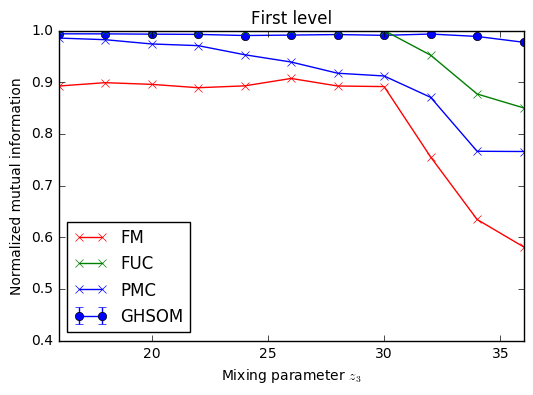
\includegraphics[width=\textwidth]{../first_level.png}
		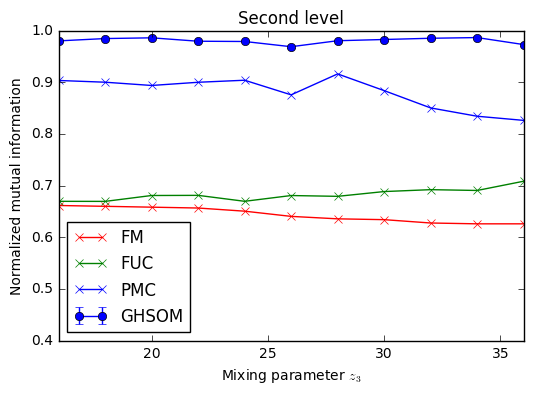
\includegraphics[width=\textwidth]{../second_level.png}
		\caption{Plot of mixing parameter $z_3$ against NMI score for both levels of community. 100 networks were generated with each mixing parameter. Results extracted without permission from \protect\cite{yang2013hierarchical} (fig 4).}
		\label{synthetic_experiment}
	\end{figure}
	
	\section{Dependence upon Parameter Settings}
	After some experimentation, it became apparent that the performance of the algorithm depended greatly upon parameter settings. 
	
	
	Bayesian optimization \cite{snoek2013bayesian} software was used to find the optimal parameter settings for each real world network. \Cref{spearmint} shows the settings found and the NMI scores achieved. 
	Spearmint does not record the random seed that generated these results so they are merely used here as an indication of the potential of GHSOM. 
	Optimization achieved good results compared to the results found in the literature and so some time was spent attempting to make the setting of parameters more principled.
	
	\begin{table}
		\centering
		\begin{tabular}{p{1.95cm} l l l l}
			\toprule
			\textbf{Parameter} & \multicolumn{4}{c}{\textbf{Network}} \\
			{} & Karate & Dolphin & Polbook & Football \\
			\bottomrule
			\textbf{\#jobs} & 28 & 521 & 562 & 181 \\
			\bottomrule
			$\eta$ & 0.0001 & 0.879 & 0.999 & 0.0587 \\
			$\sigma$ & 0.817 & 0.001 & 0.650 & 1.0 \\
			$\epsilon_{sg}$ & 0.988 & 0.558 & 1.0 &  0.451 \\
			$\epsilon_{en}$ & 1.0 & 0.3 & 0.393 & 0.3 \\
			\bottomrule
			\textbf{\#comms} & 2 & 4 & 3 & 12 \\
			\textbf{\#comms det.} & 2 & 4 & 2 & 11 \\
			\textbf{NMI score} & 1.0 & 0.640 & 0.688 & 0.874 \\
			\bottomrule
		\end{tabular}
		\caption{Spearmint optimized parameter settings and NMI scores for real world networks (to 3 s.f.). \textbf{\#jobs} is the number of completed jobs before the NMI score was recorded. Maps were trained for $\lambda=1000$ training epochs before calculating quantization error.}
		\label{spearmint}
	\end{table}
	
 
	Since one neuron in the map corresponds to one community in the network, and we desire the final number of neurons in the map to be equal to the number of communities in the data, the investigation focussed on $\epsilon_{sg}$, which controlled final map size. 
	
	%TODO
	In order to make the choice of setting $\epsilon_{sg}$ more principled, an experiment was devised to measure the impact of community size on the best choice of $\epsilon_{sg}$. Synthetic networks were generated with $c\in[3,6]$ communities. $\epsilon_{sg}$ varied varied over the interval $[0.5, 1.0]$ and the setting with the best mean NMI score over 10 repeats was recorded. \Cref{parameter_experiment} shows the results of this experiment. Since, in general, we do not know the number of communities in a network a-priori, the experiment was repeated, this time measuring network density $\rho$, a measure that is simple to calculate for any network in terms of number of nodes $n$ and number of edges $m$ as 
	\begin{align*}
	\rho = \frac{2 m}{n (n - 1)}
	\end{align*}
	
	\Cref{density} shows a plot of the result of this experiment. 
	
	\begin{figure}
		\centering
		\begin{tabular}{c c c c c}
			\toprule
			$\epsilon_{sg}$ & \multicolumn{4}{c}{\textbf{\#communities}} \\
			{} & 3 & 4 & 5 & 6 \\
			\bottomrule
			0.5 & 0.567 & 0.900 & 0.978 & \textbf{0.987} \\
			0.6 & 0.601 & 0.965 & \textbf{0.981} & 0.952 \\
			0.7 & 0.746 & \textbf{0.977} & 0.912 & 0.931 \\
			0.8 & 0.763 & 0.974 & 0.947 & 0.953 \\
			0.9 & \textbf{0.889} & 0.843 & 0.856 & 0.827 \\
			1.0 & 0.209 & 0.119 & 0.208 & 0.335 \\
			\bottomrule
		\end{tabular}
		\caption{Community size against setting of $\epsilon_{sg}$. Communities contained 32 nodes and each node has 16 connections to nodes within its own community, and 16 to nodes outside. NMI scores in bold show the best NMI score for the number of communities. Each setting was repeated 10 times. }
		\label{parameter_experiment}
	\end{figure}
	
	\begin{figure}
		\centering
		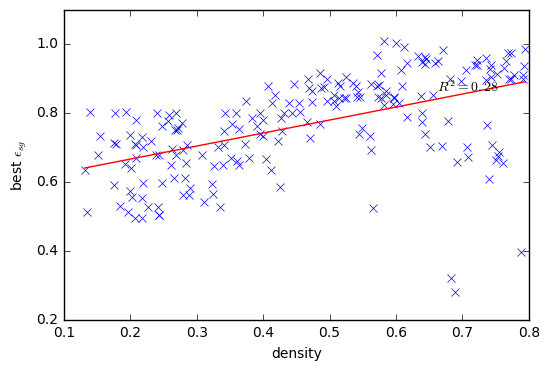
\includegraphics[width=\textwidth]{../derived_results.png}
		\caption{Plot of network density vs. best setting for $\epsilon_{sg}$. 200 random networks of 64 nodes were generated with a random number of edges and communities.}
		\label{density}
	\end{figure}
	


	The experiments did not seem to show any significant correlations and so investigation into deriving a principled method of parameter setting was dropped, in favour of more a productive (and interesting) research goal.
	
	
	\chapter{Functional Similarity of Neighbouring Communities}
	
	Each neuron on the map represents one community in the original complex network. And, due to the topology preserving property of SOM, adjacent neurons in the map represent adjacent communities (see \cref{colouring}). Since, in complex networks, a community can have some real world meaning, then a natural question to ask is whether neighbouring communities interact (or even co-operate) in their function. Experiments were undertaken to investigate this. 
	
	\begin{figure}
		\centering
		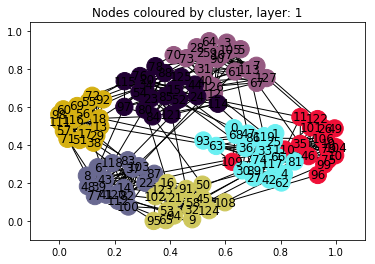
\includegraphics[width=\textwidth]{../figure2_network.png}
		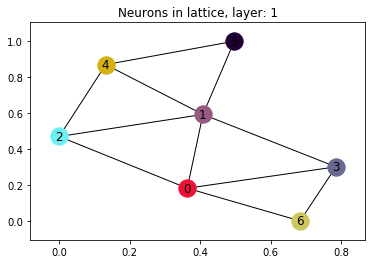
\includegraphics[width=\textwidth]{../figure2_map.png}
		\caption{Visualisation of simple generated network and resulting map. Nodes are coloured in the network by the neuron in the map that they are assigned to.}
		\label{colouring}
	\end{figure}
	
	\section{Background: The Gene Ontology}
	
	The Gene Ontology (GO) provides a controlled universal vocabulary for the communication known information about genes across all \textit{eukaryotes} (organisms with cells containing a nucleus) \cite{ashburner2000gene}. It is accessible world wide via the internet and update constantly as new discoveries are made by researchers. It is represented as three directed acyclic graphs (DAGs) that correspond to the three ontologies: Biological Process (BP), Molecular Function (MF), and Cellular Component (CC). Nodes on the DAG correspond to GO terms that are used to annotate genes through the use of annotation databases. Edges are the relationships between terms. The most common relationship is the \textit{"is a"} relationship, but there is also the \textit{"is part"}, \textit{"has part"} and \textit{"regulates"} relationships. The three ontologies are largely unconnected, with the exception of \textit{"regulates"} relationships. Each relationship requires a different form of logical reasoning. These ontologies obey the true path rule in that if a gene is annotated with a particular GO term then its is automatically annotated with all of the parents of that term right to the root of the ontology.
	
	\begin{figure}
		\centering
		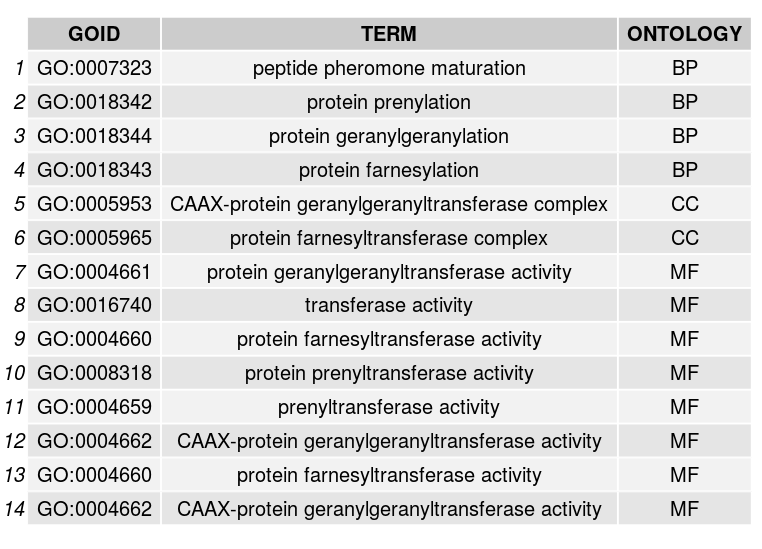
\includegraphics[width=\textwidth]{../go_terms_YKL019W.png}
		\caption{All GO terms annotated to the gene with OPF identifier YKL019W in the org.Sc.sgd.db annotation database. YKL019W is automatically annotated with the parents of all these terms due to the true path rule of GO.}
		\label{all_go_YKL019W}
	\end{figure}
	
	\begin{figure}
		\centering
		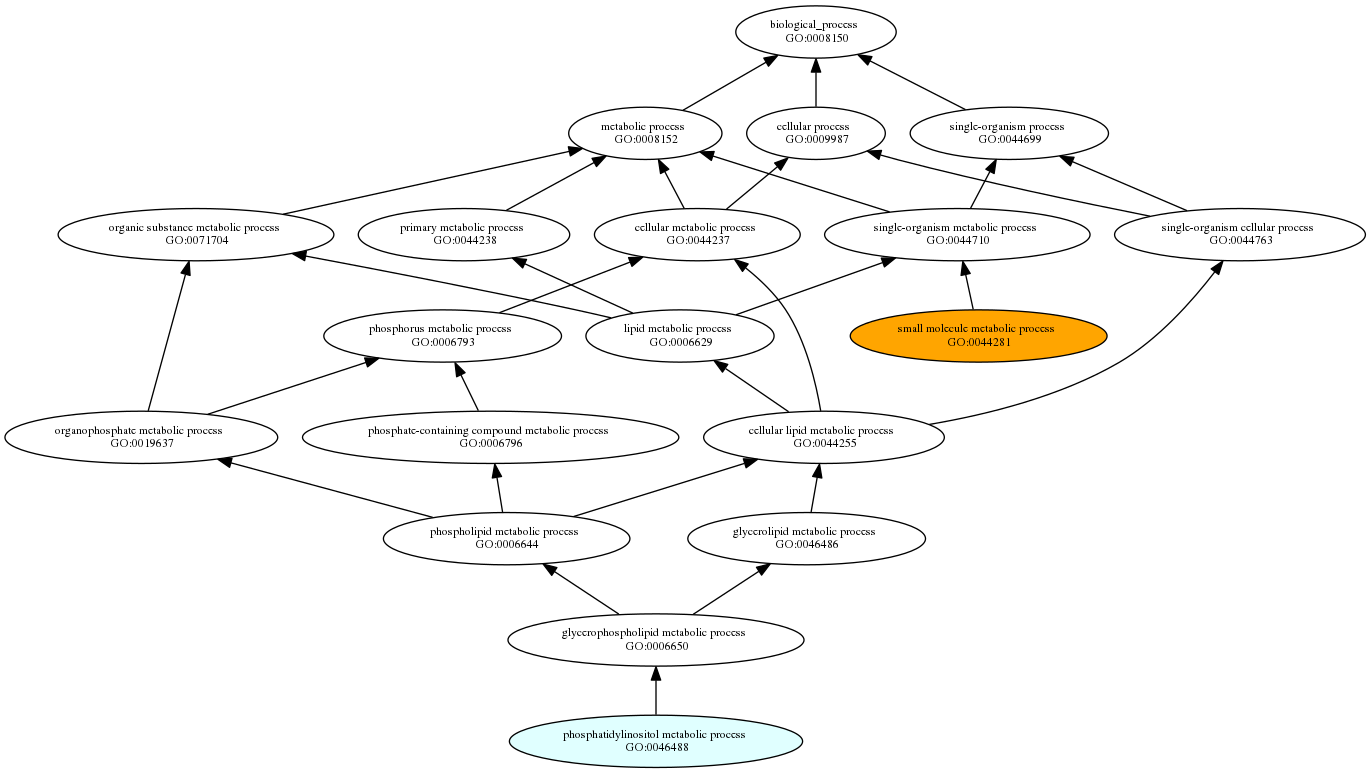
\includegraphics[width=\textwidth]{../go_term_graph.png}
		\caption{Relative positions of the terms GO:0044281 \textit{small molecule metabolic process} and GO:0046488 \textit{phosphatidylinositol metabolic process} in the Biological Process (BP) ontology. Graph generated using the web tool G-SESAME \protect\cite{du2009g}.}
		\label{go_term_graph}
	\end{figure}
	
	\section{Experiments on Saccharomyces Cerevisiae dataset}	

	
	Two Saccharomyces Cerevisiae (budding yeast) network data sets were used. \Cref{yeast_networks} details the size of the networks. 
		
	\begin{table}
		\centering
		\begin{tabular}{c c c}
			\toprule
			\textbf{Network name} & \textbf{Number of Nodes} & \textbf{Number of Edges} \\ \bottomrule
			Uetz Screen & 263 & 292 \\
			Y2H Union & 1647 & 2682 \\ \bottomrule
		\end{tabular}
		\caption{Topology information for the two Saccharomyces Cerevisiae networks. Datasets available from \protect\cite{uetz,union}.}
		\label{yeast_networks}
	\end{table}
	
	\begin{figure}
		\centering
		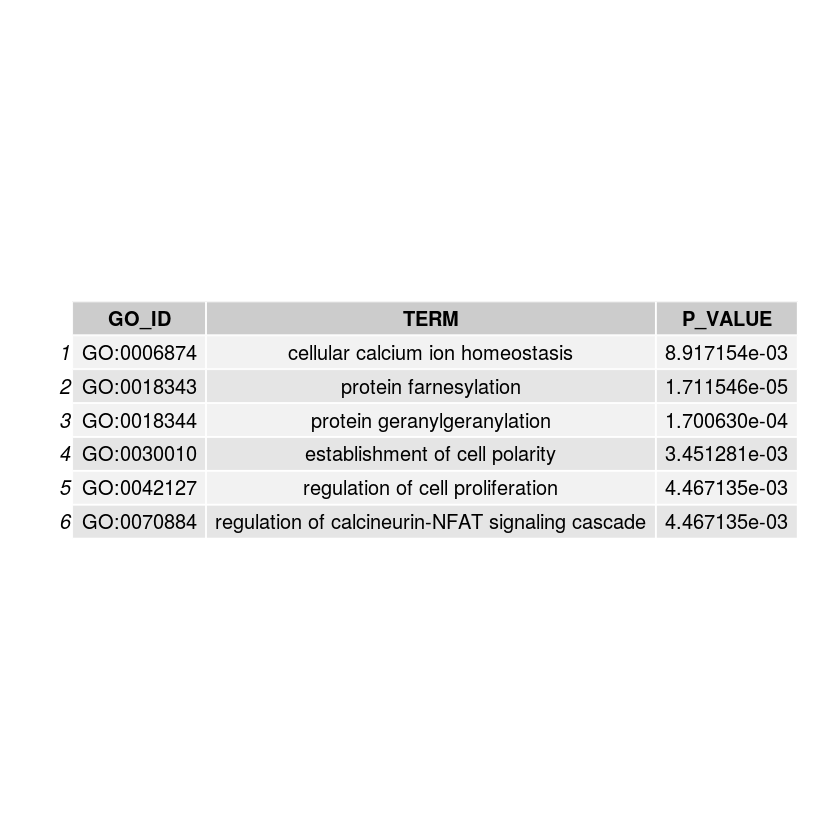
\includegraphics[width=\textwidth]{../enriched_go_terms.png}
		\caption{Enriched GO terms (p-value $<$ 0.01) in the BP ontology and their respective p-values for the genes with ORF identifiers: YKL019W, YGL155W, KL159C, YCR063W, YBR247C, YDL090C, YOL135C. Table generated using the R package GOSim \protect\cite{frohlich2007gosim} which is built upon topGO \protect\cite{alexa2010topgo}.} 
		\label{gosim_enriched_gos}
	\end{figure}
	
	After the networks are partitioned into communities by GHSOM, the set of enriched GO terms (p-value $<$ 0.01) for each community was computed, using GO annotations from the org.Sc.sgd.db annotation database. The p-value was computed from a 2x2 contingency table and corresponded to the probability of the observed distribution of genes labelled with a particular GO term occurring from a random sample of genes drawn from the population. \Cref{cont_table} gives an example of one such table.

	
	\begin{figure}
		\centering
		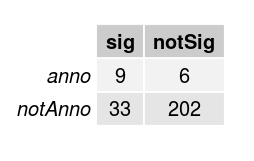
\includegraphics[width=\textwidth]{../contingency_table.png}
		\caption{An example contingency table for the go term: GO:0006914 \textit{autophagy} (Fisher's exact test p-value=0.000111024375808973).}
		\label{cont_table}
	\end{figure}
	
	Two semantic similarity measures found commonly in the literature were used in this work. Resnik and Wang.
	
	
	\subsection{Resnik}
	
	The Resnik measure was first used to compute the semantic similarity of words \cite{resnik1999semantic}. It involves computing the `frequency' of a term as 
	
	\begin{align}
	p(t) = \frac{|\{t, \text{children of } t\}|}{N}
	\end{align}
	
	which is used to assign a measure of information content (IC) to each term in the ontology:
	
		
	\begin{align}
	\text{IC}(t) = -log(p(t))
	\end{align}
	
	This ensures that terms with few children contain more information.

	The Resnik measure assigns similarity equal to the maximum information content of a common parent of both terms in in the ontology. Terms that are more related will have common parents further down the tree and these parents will have a higher IC. Sevilla et al. found that ``Resnik's measure correlates well with gene expression'' \cite{sevilla2005correlation}.
	
	\begin{align}
	\text{sim}_{RESNIK}(t_1, t_2) = \max_{i \in \{\text{parents of }t_1\} \cap \{\text{parents of } t_2\}}(\text{IC}(i))
	\end{align}
	
	To calculate the similarity of two gene sets, the Best Match Average (BMA) method is used. One first finds the enriched GO terms and then computes the pairwise similarity between each term in both sets. The best match for each row and column is summed and divided by the number of rows and columns.
	
	\begin{align}
	\text{sim}_{BMA}(G_1, G_2) = \frac{\sum_{i = 1}^{m} \max_{1\leq j\leq m} sim(G_{1i}, G_{2j}) + \sum_{j = 1}^{n} \max_{1\leq i\leq n} sim(G_{1j}, G_{21})}{m + n}
	\end{align}
	
	\begin{figure}
		\centering
		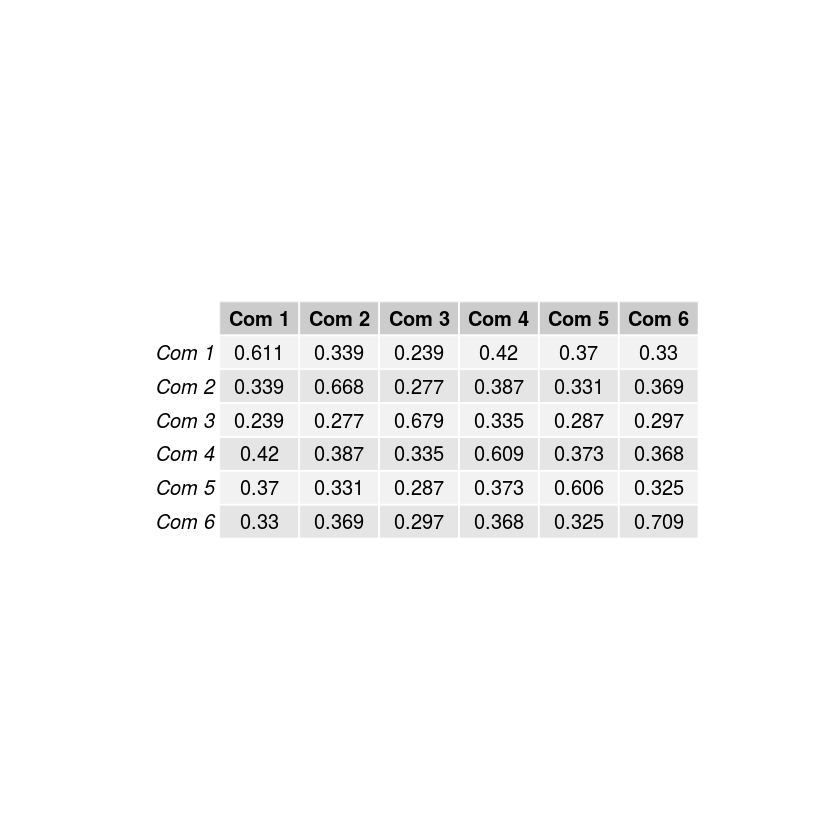
\includegraphics[width=\textwidth]{../resnik.png}
		\caption{Example similarities between the six communities discovered by GHSOM in the Uetz screen network in the MF ontology using the Resnik similarity measure.}
		\label{resnik}
	\end{figure}
	
	\begin{figure}
		\centering
		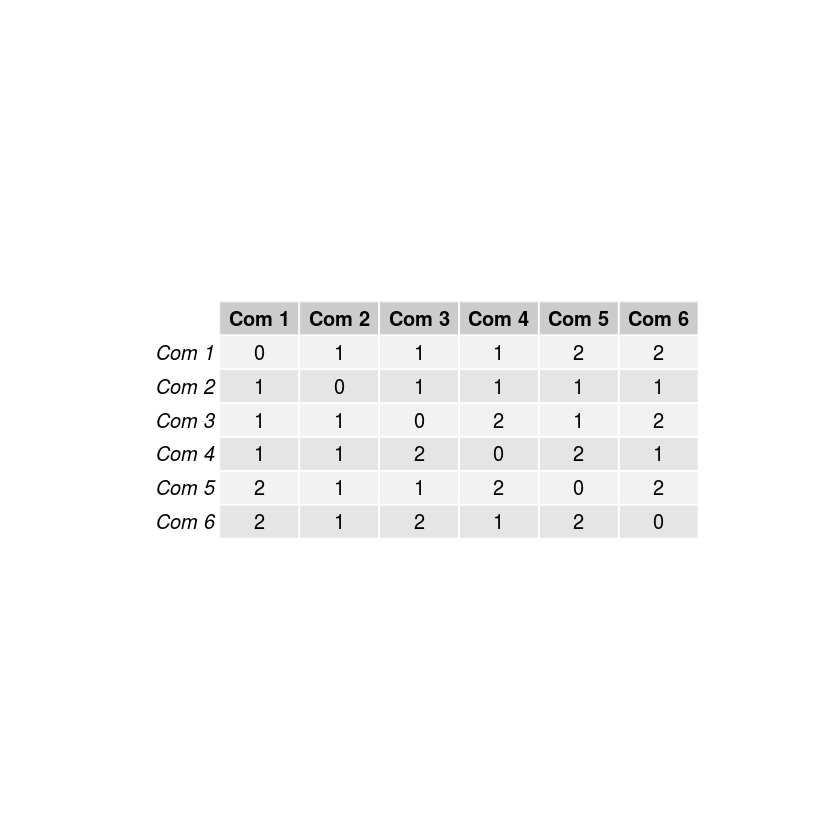
\includegraphics[width=\textwidth]{../shortest_path.png}
		\caption{Distances of neurons on the map.}
		\label{shortest_path}		
		
	\end{figure}
	

	
	\subsection{Wang}
	
	The Wang measure is based on the topology of the GO ontology itself \cite{wang2007new}. One must first assign weightings $w_e$ to each relation in the ontology. (I use $w_e=0.8$ for `is a'') and then compute the S-value of every term $t$ in the DAG $T_A$ consisting of the original term $A$ and all of its ancestors, as 
	
	\begin{align}
	S_A(t) = 
	\begin{cases}
	1, & \text{if } t = A \\
	\max\{w_e * S_A(t') | t' \in \text{children of }t\}, & \text{if }t\neq A
	\end{cases}
	\end{align} 
	
	Then we can compute the semantic value of term $A$ as 
	
	\begin{align}
	\text{SV}(A) = \sum_{t \in T_A} S_A(t)
	\end{align}
	
	Finally, the similarity of two terms is
	
	\begin{align}
	sim_{WANG}(A, B) = \frac{\sum_{t\in T_A \cap T_B}  S_A(t) + S_B(t)}{\text{SV}(A) + \text{SV}(B)}
	\end{align}
	
	
	\begin{figure}
		\centering
		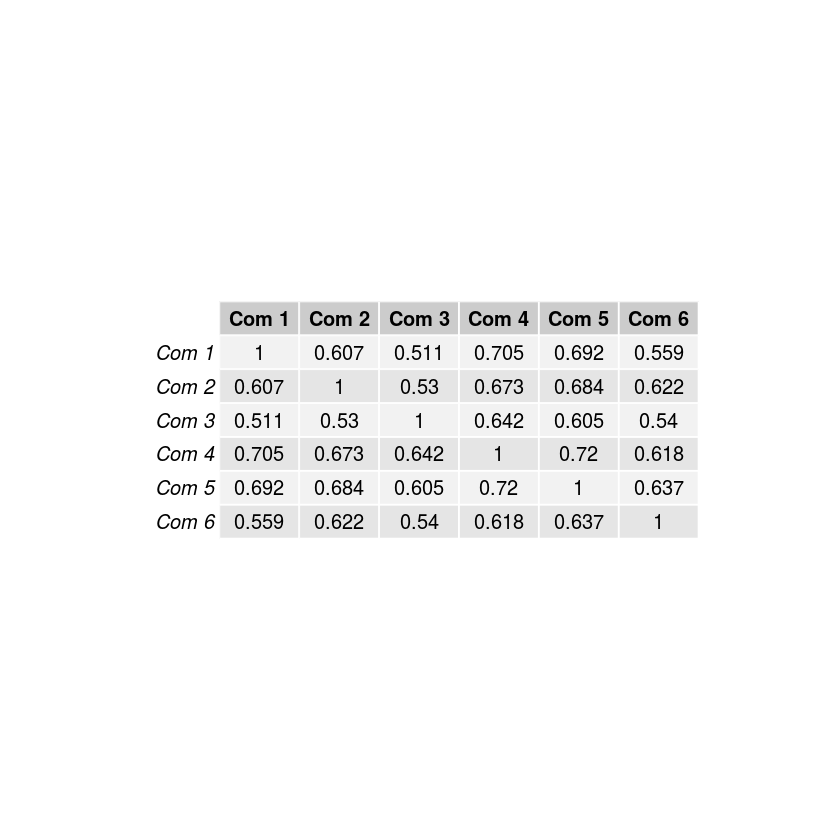
\includegraphics[width=\textwidth]{../wang.png}
		\caption{Example similarities between the six communities discovered by GHSOM in the Uetz screen network in the MF ontology using the Wang similarity measure.}
		\label{wang}
	\end{figure}
	
	\begin{figure}
		\centering
		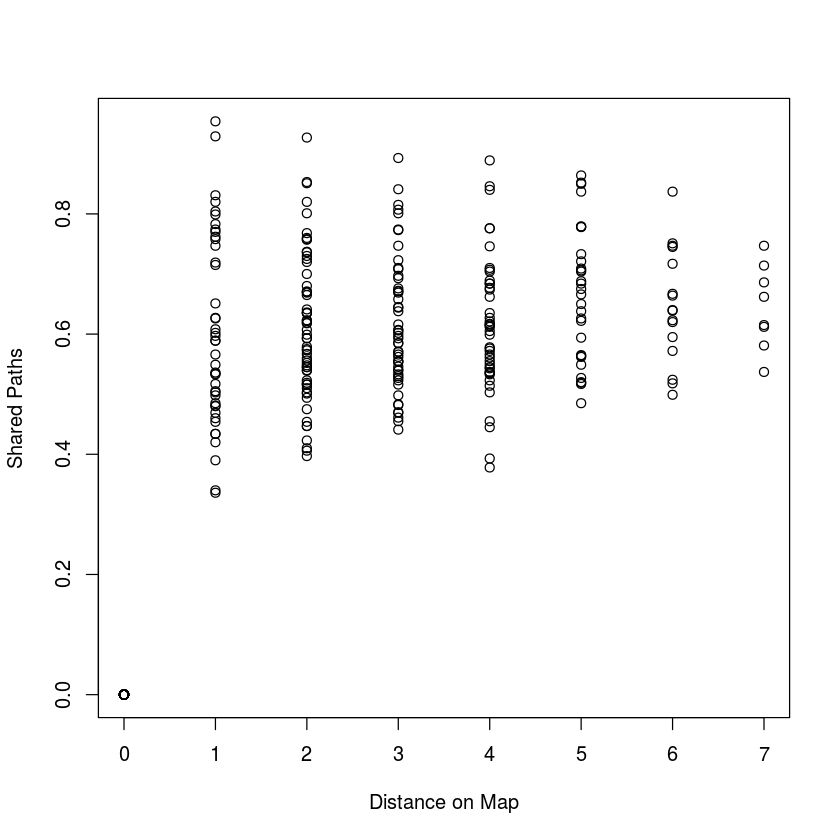
\includegraphics[width=\textwidth]{../semantic_results.png}
		\caption{Plot of semantic similarity against distance of map using the Wang measure on the Y2H Union dataset.}
		\label{semantic_results}
	\end{figure}
	
%	\section{Embedding based on Functional Similarity}
	
	%TODO maybe get something interesting here?

	\chapter{Discussion \& Future Plans}

	The aim of my study was to investigate the usefulness of GHSOM as a tool for hierarchical community detection. 
	We found that GHSOM was capable of community detection on both small real world and synthetic networks. 
	With some optimization, GHSOM was able to produce results as good as the other algorithms in the literature on the real world networks (\cref{bayes}). However, the results achieved by the spearmint software are difficult to reproduce and seem to rely heavily on a lucky random initialization.
	
	On the synthetic experiments, GHSOM consistently achieved almost perfect NMI scores for both level of community, even when the external degree of nodes was greater than the internal degree (\cref{synthetic_experiment}).
	Both \cite{lancichinetti2009detecting} and \cite{yang2013hierarchical} struggled with these cases and the NMI score for $z_3 > 32$ dropped noticeably (to less than 0.9).
	%TODO WHY?
	In this author's opinion, this is the result of embedding using MDS. In the cases of $z_3 > 32$, each node had 16 connections to nodes in the same micro community (31 other nodes), 16 connections to nodes in the same macro, but not micro community (96 other nodes) and 32-36 connections to the 384 nodes of the network. 
	Even though the external degree of each node was greater than the internal degree, the ratio of connections to possible target nodes was still decreasing.
	Because of this, the distance between nodes of different communities was still larger than nodes of the same community and so MDS was able to embed these nodes in such a way that identifying communities was still possible. 
	Bonabeau \cite{bonabeau2002graph} cites \cite{kernighan1970efficient} who identified that MDS can allow for clusters and communities within a graph to be more easily identifiable even before a cover is found. 
	
	The semantic similarity measures have not yet shown any correlation between community distance on the map (see \cref{semantic_results} for an example) and I would like to spend a little more time investigating this. I would also like to investigate the similarity of neighbouring communities in social networks. 
	
	Another area I would like to investigate before completing this work is to embed the genes based on semantic similarity with each other (rather than shortest path distance on the network) and explore the clusters discovered by GHSOM in this case. Since the embeddings are not based on topology, there is not guarantee that neighbouring nodes on the graph will be embedded together and so the clusters may not represent true communities but functional clusters.  
	
	At the end of my work on GHSOM, I would like to continue working on topographic feature selection, but using a semi-restricted Boltzmann machine, with interlayer links on the hidden layer to uncover the relationships between the learned features. I have taken some time to implement a working RBM that runs efficiently on the GPU as a starting point for my experimentation with this. In general, I would like to build some generative model to infer the underlying features of the network, and use this model to uncover more powerful features than features based on topology alone. 
	
	\bibliography{../references}
	\bibliographystyle{unsrt}
	
\end{document}